\documentclass[12pt]{beamer}

\usepackage[UTF8]{ctex}
\usepackage{bm}
\usepackage{cleveref}
\usepackage{hyperref}
\usetheme[progressbar=frametitle]{metropolis}

\usepackage{amsmath,amssymb,enumerate,color}
\usepackage{graphicx,listings}

\definecolor{light-gray}{gray}{0.95} 
\lstset{ %
	backgroundcolor=\color{light-gray},   % choose the background color
	basicstyle=\scriptsize\rmfamily,     % size of fonts used for the code
	columns=fullflexible,
	breaklines=true,                 % automatic line breaking only at whitespace
	captionpos=b,                    % sets the caption-position to bottom
}

\begin{document}

\section{代数方程的求解}
	\subsection{代数方程的图解法}
\begin{frame}[fragile]{一元方程的图解法}
		  	\textbf{思路:}用ezplot()函数绘隐函数$f(x)=0$曲线找零点。
			 \begin{example}[6-1]
				解$\mathrm{e}^{-3 t} \sin (4 t+2)+4 \mathrm{e}^{-0.5 t} \cos (2 t)=0.5$。

		  	\begin{columns}[T]
			  		\column{.4\textwidth}
			  	\begin{block}{MATLAB代码:}
    \begin{lstlisting}
figure
ezplot('exp(-3*t)*sin(4*t+2)+4*exp(-0.5*t)*cos(2*t)-.5',[0 5])
line([0,5],[0,0])
    \end{lstlisting}	
			\end{block}	  		
		  		\column{.6\textwidth}
				\begin{block}{输出:}
					\centering
					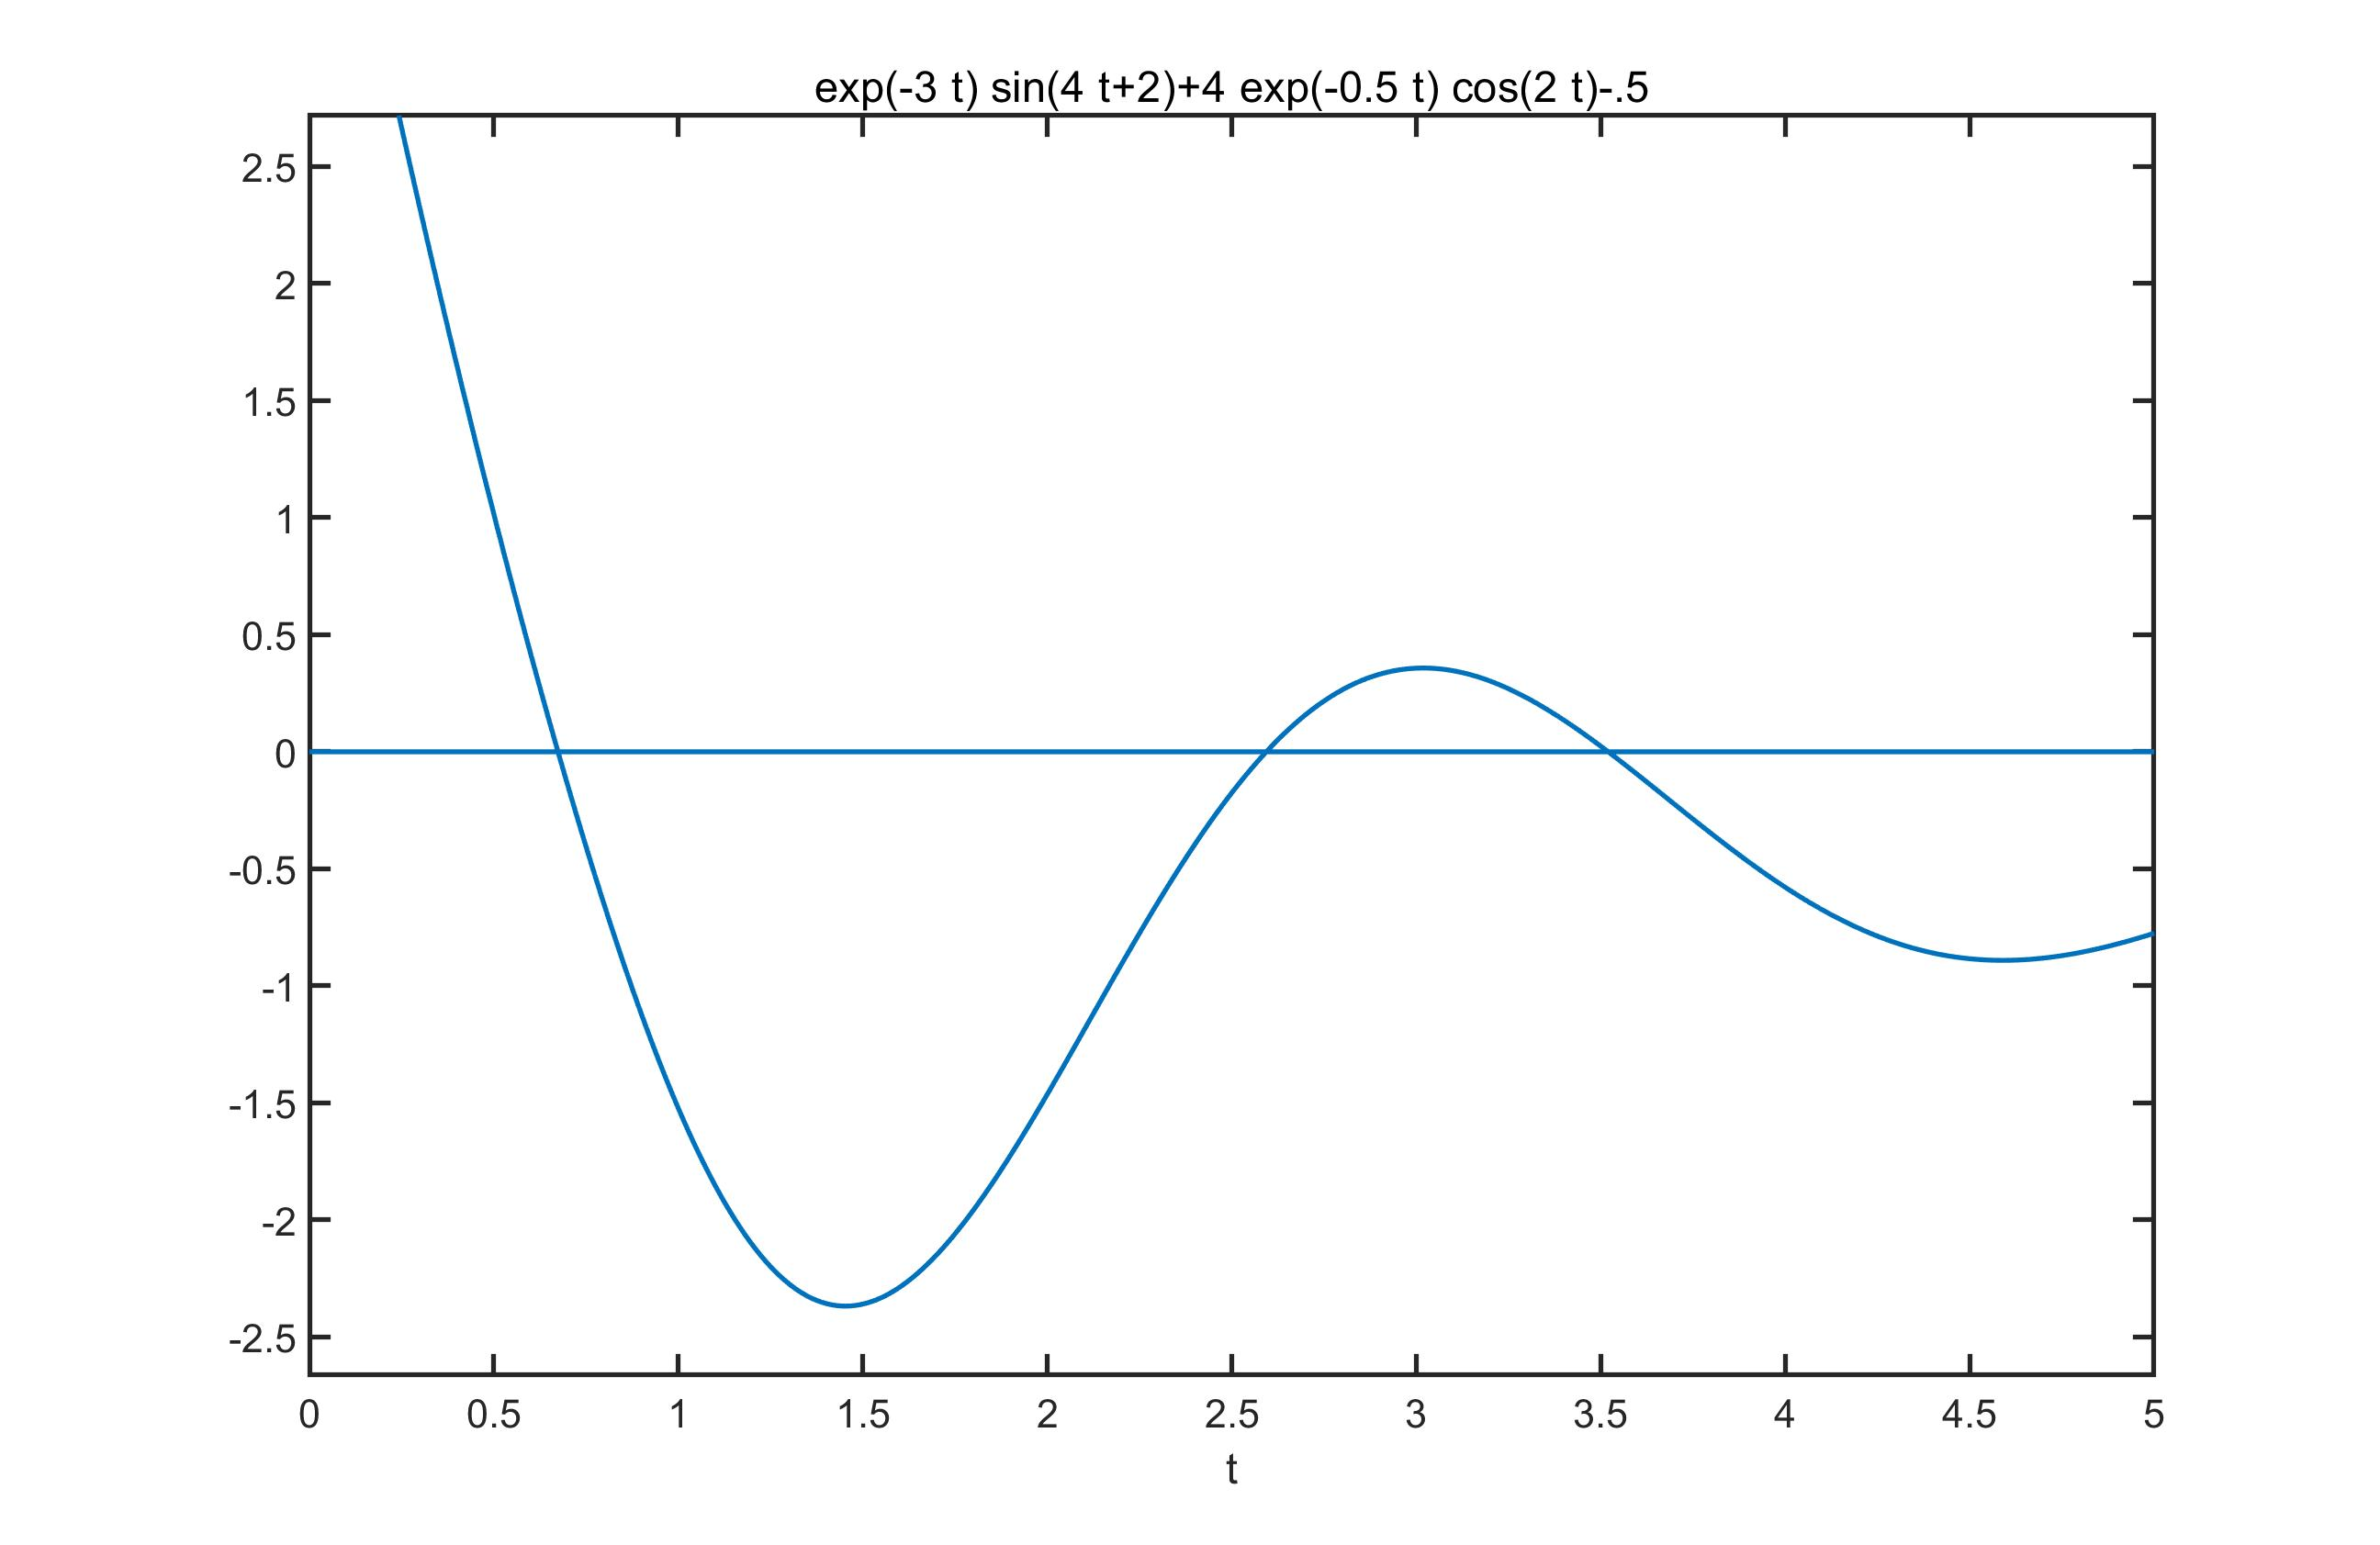
\includegraphics[width=\textwidth]{11}
				 \end{block}
		  	\end{columns}
三个解,约为0.670、2.59、3.51.
		\end{example}
\end{frame}
%---------------------------------------------------------------------- 	
\begin{frame}[fragile]{二元方程的图解法}
		\textbf{思路:}绘制在同一张图上看交点。
	\begin{example}[6-2]解
		$\left\{\begin{array}{l}
		x^{2} \mathrm{e}^{-x y^{2} / 2}+\mathrm{e}^{-x / 2} \sin (x y)=0 \\
		x^{2} \cos \left(x+y^{2}\right)+y^{2} \mathrm{e}^{x+y}=0
		\end{array}\right.$
	
		\begin{columns}[T]
			\column{.4\textwidth}
				\begin{block}{MATLAB代码:}
\begin{lstlisting}
figure
ezplot('x^2*exp(-x*y^2/2)+exp(-x/2)*sin(x*y)')
hold on
h1 = ezplot('y^2*cos(y+x^2)+x^2*exp(x+y)');
set(h1,'Color','k')
hold off
\end{lstlisting}
				\end{block}	  		
		
			\column{.6\textwidth}
				\begin{block}{输出:}
					\centering
					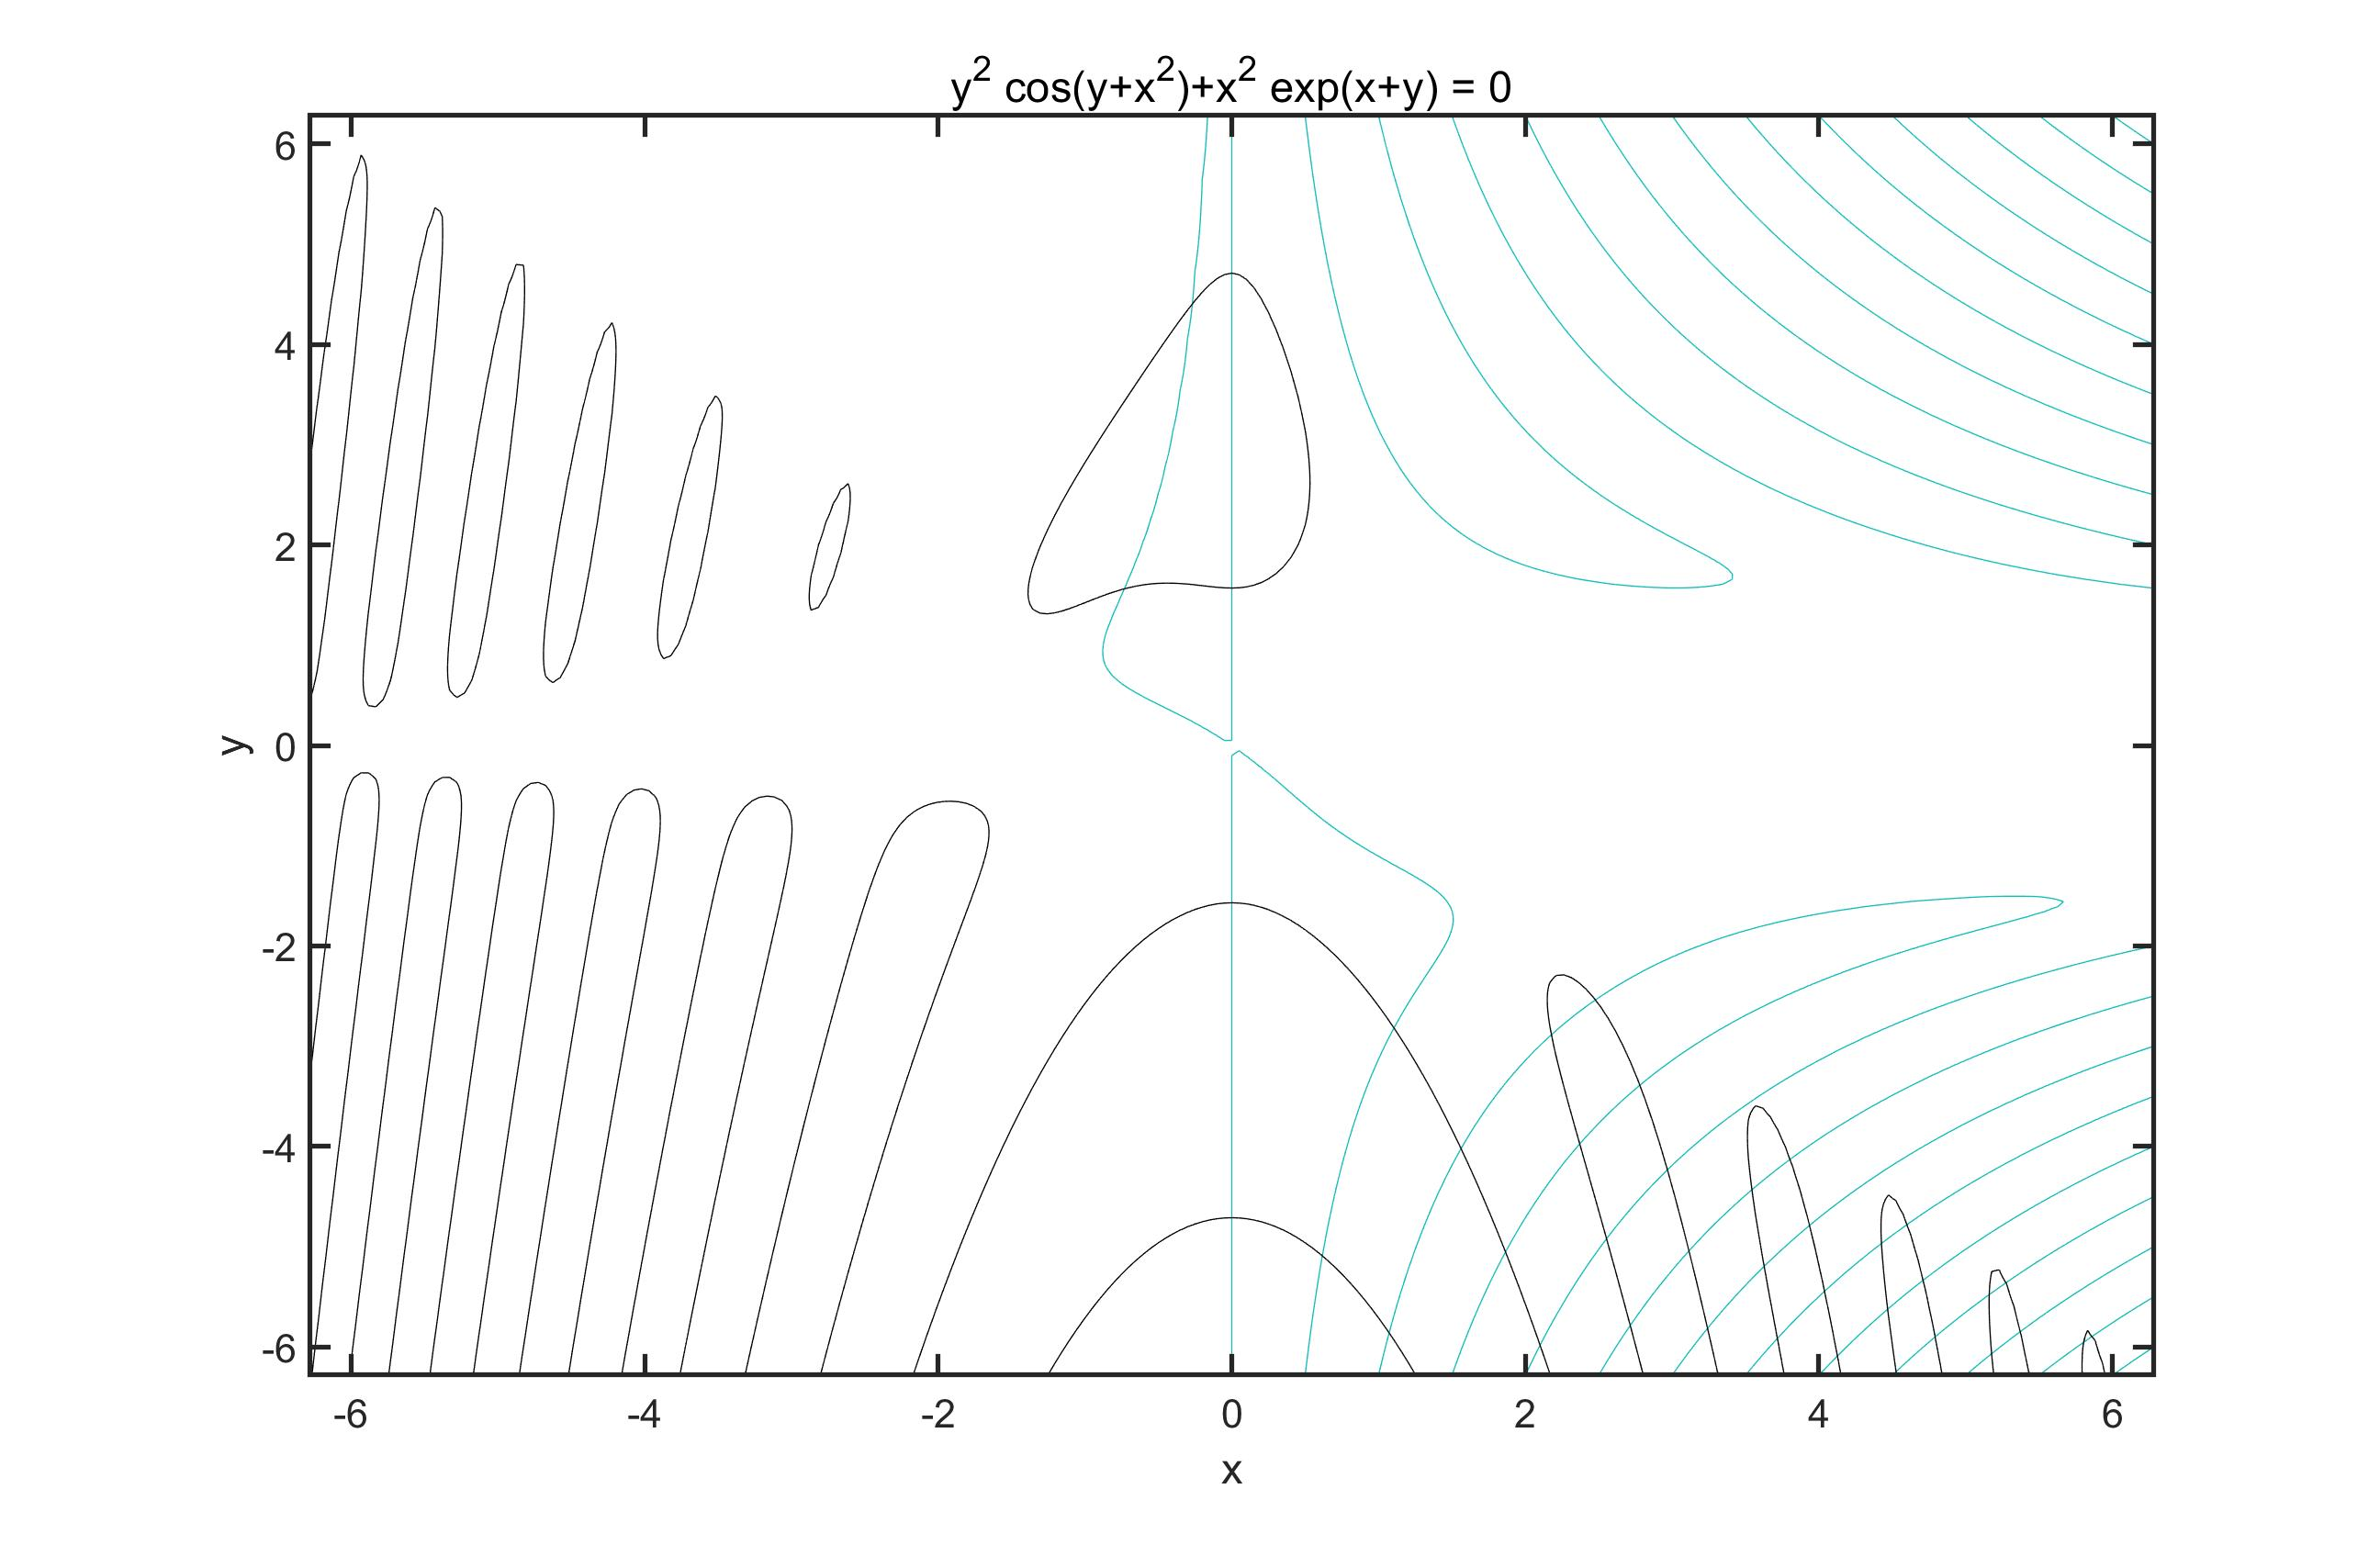
\includegraphics[width=\textwidth]{12}
				\end{block}
		\end{columns}
	\end{example}

	\textbf{局限:}
仅适用\textbf{一元、二元}方程。
仅能\textbf{近似}得\textbf{实数}根。

\end{frame}
%---------------------------------------------------------------------- 
	\subsection{多项式型方程的准解析解法}
		\begin{frame}[fragile]{多项式型方程的准解析解法}
		\begin{block}{用solve函数,语法:}
\begin{lstlisting}
S = solve(eqn1, eqn2,... ,eqnn)%最简调用方式
[x,...] = solve(eqn1, eqn2,... ,eqnn)%直接得出根
[x,...] = solve(eqn1, eqn2,... ,eqnn, 'x,...')%同上, 并指定变量
\end{lstlisting}
		\end{block}	  
		\begin{columns}[T]
			\column{.7\textwidth}
		\begin{example}[6-4]
			解$\left\{\begin{array}{l}
			x^{2}+y^{2}-1=0 \\
			0.75 x^{3}-y+0.9=0
			\end{array}\right.$
		\end{example}
	\begin{block}{MATLAB代码:}
\begin{lstlisting}
syms x y
[x,y]=solve(x^2+y^2-1==0,0.75*x^3-y+0.9==0)
x=double(x), y=double(y)
[eval('x.^2+y.^2-1') eval('0.75*x.^3-y+0.9')]%解的验算
\end{lstlisting}
	\end{block}
			\column{.3\textwidth}
		\begin{block}{输出:}
\begin{lstlisting}
x = -0.9817 + 0.0000i
    0.3570 + 0.0000i
    -0.5540 - 0.3547i
    -0.5540 + 0.3547i
    0.8663 - 1.2154i
    0.8663 + 1.2154i
y = 0.1904 + 0.0000i
    0.9341 + 0.0000i
    0.9293 - 0.2114i
    0.9293 + 0.2114i
    -1.4916 - 0.7059i
    -1.4916 + 0.7059i
\end{lstlisting}	
		\end{block}			
	\end{columns}
		\end{frame}
%---------------------------------------------------------------------- 
	\subsection{一般非线性方程数值解}
		\begin{frame}[fragile]{一般非线性方程数值解}
	\begin{block}{用fsolve()函数,语法:}
\begin{lstlisting}
x = fsolve(fun,x0)%最简单求解语句
[x,f,flag,out] = fsolve(fun,x0,opt,p1,p2,...)%一般求解格式
opt = optimset%获得默认的常用变量
opt.TolX=1e-10; set(opt,'TolX',1e-10)%修改参数
\end{lstlisting}
	\end{block}	  

	\begin{example}[6-8]
解Lambert函数,其解$w$满足$we^{w} = x$。
	\end{example}

	\begin{block}{MATLAB代码:}
		\begin{columns}[T]
	\column{.5\textwidth}
\begin{lstlisting}
figure
y=[]; xx=0:.05:10; x0=0; h=optimset; h.Display='off';
for x = xx
y1 = fsolve(@(w) w.*exp(w)-x,x0,h); x0=y1; y=[y,y1];
end
\end{lstlisting}

	\column{.5\textwidth}
\begin{lstlisting}
subplot(2,1,1);
plot(xx,y);
y0 = lambertw(xx);
subplot(2,1,2);
plot(xx,y0,'r');
\end{lstlisting}
		\end{columns}
	\end{block}
\end{frame}
%---------------------------------------------------------------------- 
\begin{frame}[fragile]{一般非线性方程数值解}
	\begin{block}{输出:}
		\centering
		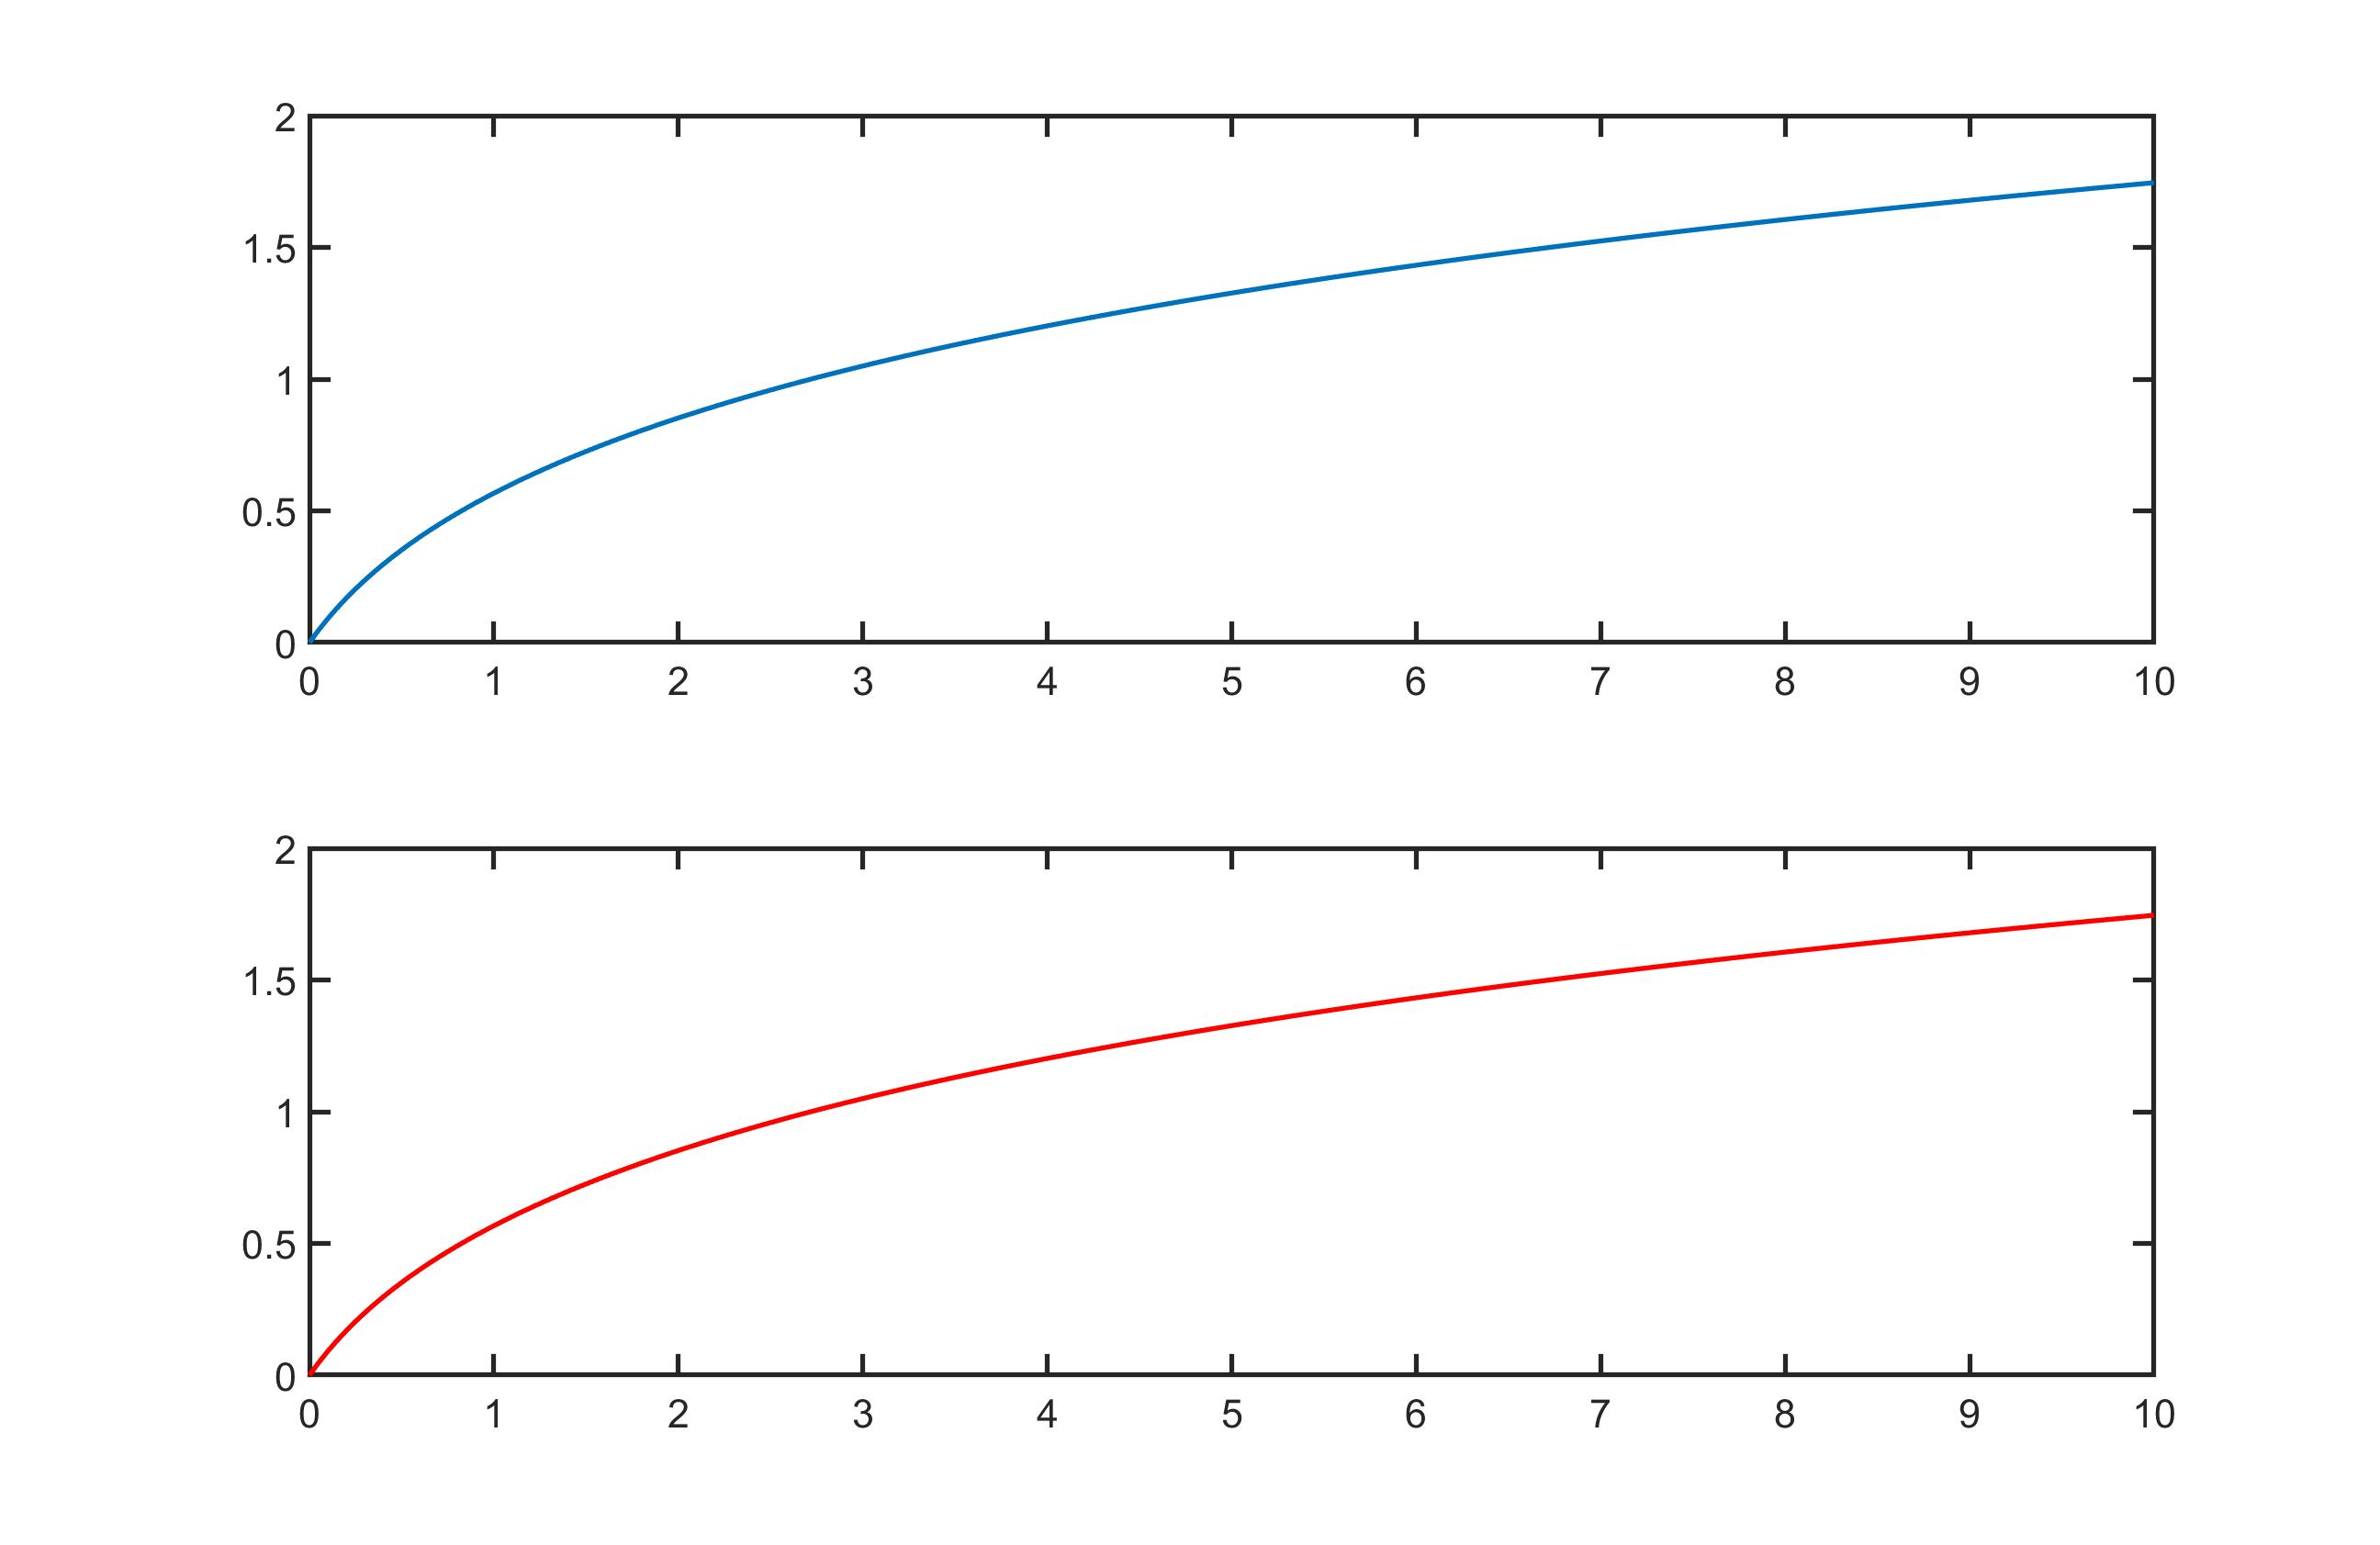
\includegraphics[width=.7\textwidth]{13}
		
		{\color{cyan}蓝线}:fsolve()的解,{\color{red}红线}:软件自带该问题求值函数。
	\end{block}		
\end{frame}
%---------------------------------------------------------------------- 
\section{无约束最优化问题求解}
	\subsection{解析解法与图解法}
		\begin{frame}[fragile]{解析解法与图解法}
\textbf{无约束最优化问题提法:}$\min\limits_{x} f(\mathbf{x})$,优化变量$\mathbf{x} = [x_1,...,x_n]^T$,目标函数$f(\cdot)$。

\textbf{解析解法:}最优点出现在一阶导数为零的点上,可列$
\left.\frac{\partial f}{\partial x_{1}}\right|_{\mathbf{x}=\mathbf{x}^{*}}=0,\left.\frac{\partial f}{\partial x_{2}}\right|_{\mathbf{x}=\mathbf{x}^{*}} 0, \cdots,\left.\frac{\partial f}{\partial x_{n}}\right|_{\mathbf{x}=\mathbf{x}^{*}}=0$

$
\Longrightarrow
\left\{\begin{array}{l}
\text{高数:Hessian矩阵。} \\
\text{\textbf{图解法:}画曲线判断极值点。} {\color{red}\checkmark}
\end{array}\right.
$
			
\textbf{局限:}一元、二元函数适用,三元或多元函数无法画图表示。
		\end{frame}
%---------------------------------------------------------------------- 
\begin{frame}[fragile]{解析解法与图解法}
\begin{columns}[T]
	\column{.4\textwidth}
		\begin{example}[6-11]
			讨论例6-1函数最优性。
		\end{example}
		\begin{block}{MATLAB代码:}
\begin{lstlisting}
syms t
y = exp(-3*t)*sin(4*t+2)+4*exp(-0.5*t)*cos(2*t)-.5;
y1 = diff(y,t)
t0 = solve(y1)
b = subs(diff(y1),t,t0)
\end{lstlisting}			
		\end{block}
		
	\column{.6\textwidth}
		\begin{block}{输出:}
			\centering
			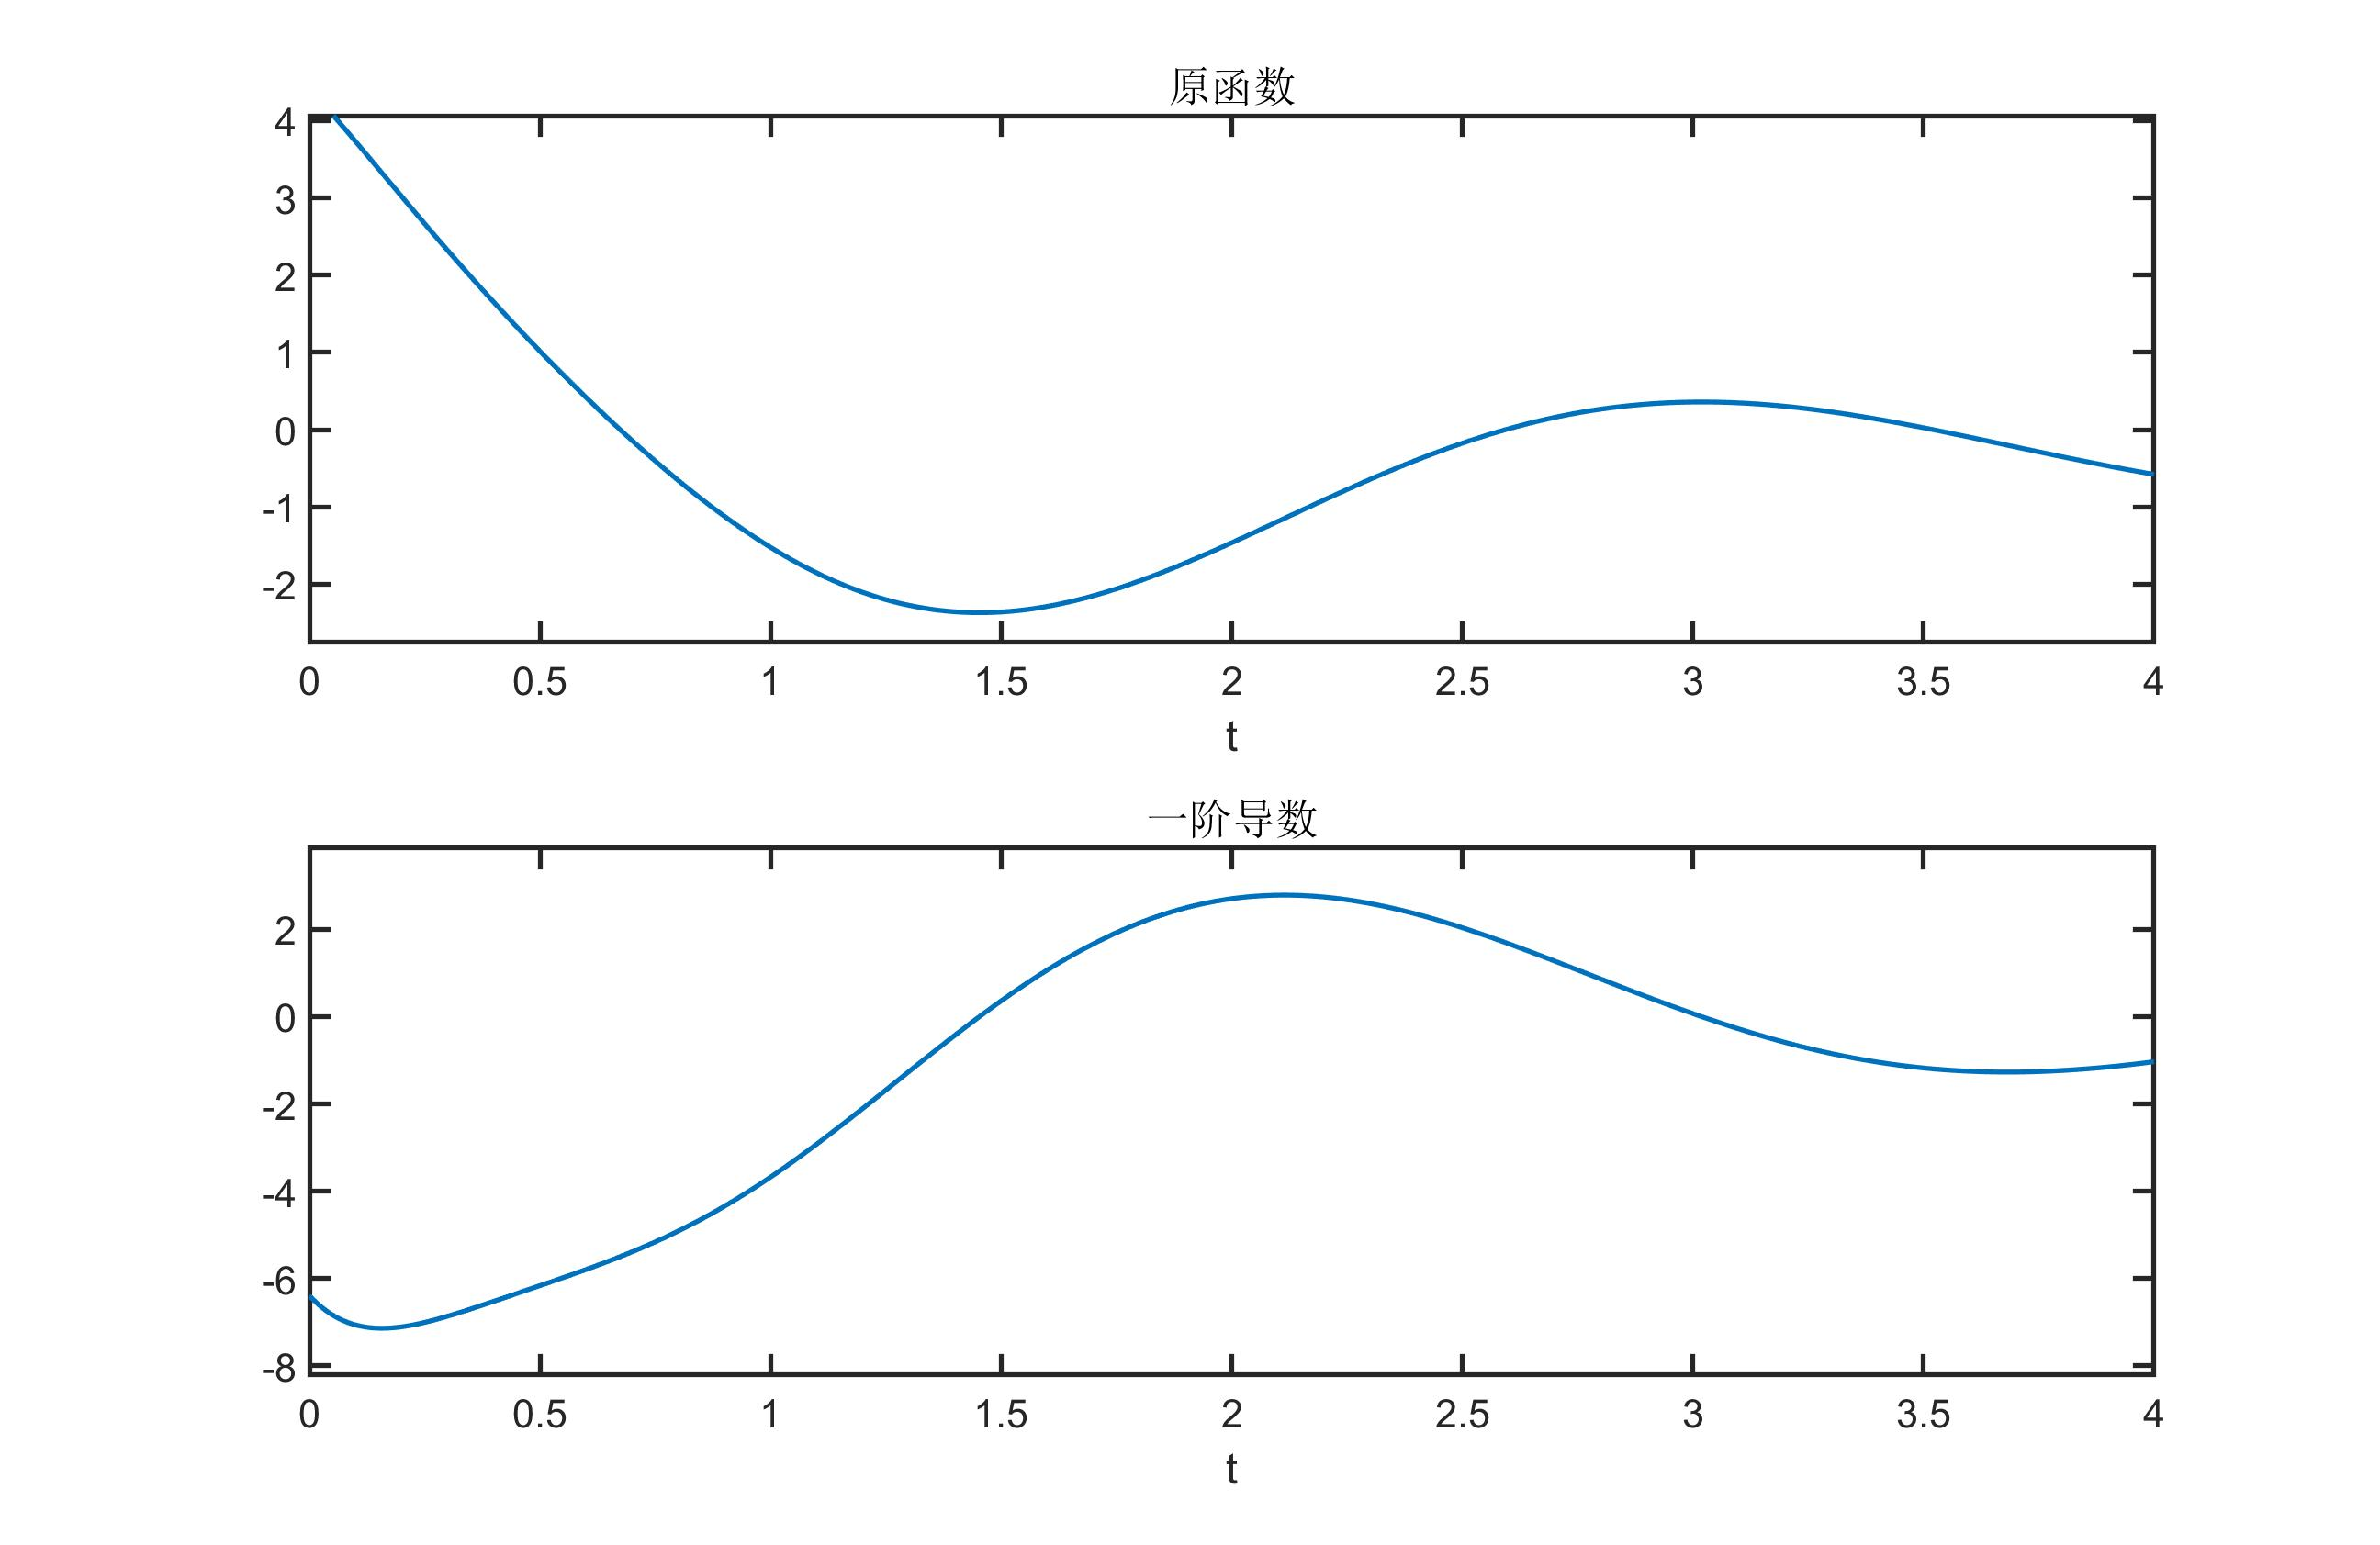
\includegraphics[width=\textwidth]{22}
			
			可见在[0,4]内约1.46处,最小值约-2.37。
		\end{block}
\end{columns}
\end{frame}
%---------------------------------------------------------------------- 
	\subsection{基于MATLAB的数值解法}
		\begin{frame}[fragile]{基于MATLAB的数值解法}
			\textbf{数学原理:}单纯形(Simplex)法。{\scriptsize(Def: N dim., N+1 vertices interconnect)}
			
			\textbf{思路:}调用fminsearch()或者fminunc()函数。
			
			\begin{block}{调用语法,fminunc()为例:}
\begin{lstlisting}
x=fminunc(Fun, x0) %最简求解语句
[x,f,flag,out]=fminunc(Fun, x0, opt, p1, p2,...) %一般求解格式
\end{lstlisting}
			\end{block}	  
		
		\begin{example}[6-12]
求$z=f(x, y)=\left(x^{2}-2 x\right) \mathrm{e}^{-x^{2}-y^{2}-x y}$最小值。
		\end{example}
			
			\begin{block}{MATLAB代码:}
\begin{lstlisting}
ff2=@(x)(x(1)^2-2*x(1))*exp(-x(1)^2-x(2)^2-x(1)*x(2));
ff2_0 = optimset;
ff2_0.Display='iter';
result1 = fminsearch(ff2,[0; 0],ff2_0)
result2 = fminunc(ff2,[0; 0],ff2_0)
\end{lstlisting}
			\end{block}	 
		
		\end{frame}
	
%---------------------------------------------------------------------- 
\begin{frame}[t,fragile]{fminsearch输出}
		
		\begin{lstlisting}
Iteration   Func-count     min f(x)         Procedure
0           1                0         
1           3     -0.000499937         initial simplex
2           4     -0.000499937         reflect
3           6      -0.00149944         expand
4           7      -0.00149944         reflect
......
71          135        -0.641424         contract inside
72          137        -0.641424         contract outside
......
优化已终止:当前的 x 满足使用 1.000000e-04 的 OPTIONS.TolX 的终止条件,F(X) 满足使用 1.000000e-04 的 OPTIONS.TolFun 的收敛条件
......
result1 =
0.6111
-0.3056
\end{lstlisting}
		
\end{frame}

%---------------------------------------------------------------------- 
\begin{frame}[t,fragile]{fminunc输出}

\begin{lstlisting}
Iteration  Func-count       f(x)        Step-size       First-order optimality
0           3                0                             2
1           6        -0.367879            0.5          0.736  
......
6          24        -0.641424              1       0.000619  
7          27        -0.641424              1        1.8e-06
......
Optimization completed because the size of the gradient is less than the value of the optimality tolerance.
......
result2 =
0.6110
-0.3055
\end{lstlisting}

\end{frame}

%----------------------------------------------------------------------
 
	\subsection{全局最优解与局部最优解}
\begin{frame}[fragile]{全局最优解与局部最优解}
	\textbf{概念:}导数为0的点包括局部和全局最优点。得到的最优点依赖于初始选取。$\Leftarrow$可以用遗传算法试不同初值
	
	\begin{columns}[T]
		\column{.4\textwidth}
		
	\begin{example}[6-13]
		$y(t)=\mathrm{e}^{-2 t} \cos 10 t+\mathrm{e}^{-3 t-6} \sin 2 t, t \geqslant 0$局部最小值与全局最小值。
	\end{example}
	
	\begin{block}{MATLAB代码:}
\begin{lstlisting}
ff3=@(t)exp(-2*t).*cos(10*t)+exp(-3*(t+2)).*sin(2*t);
[t3_1,f3_1] = fminsearch(ff3,1)
[t3_2,f3_2] = fminsearch(ff3,.1)
\end{lstlisting}
	\end{block}	
	
		\column{.65\textwidth}
		
		\begin{block}{输出:}
	\centering
	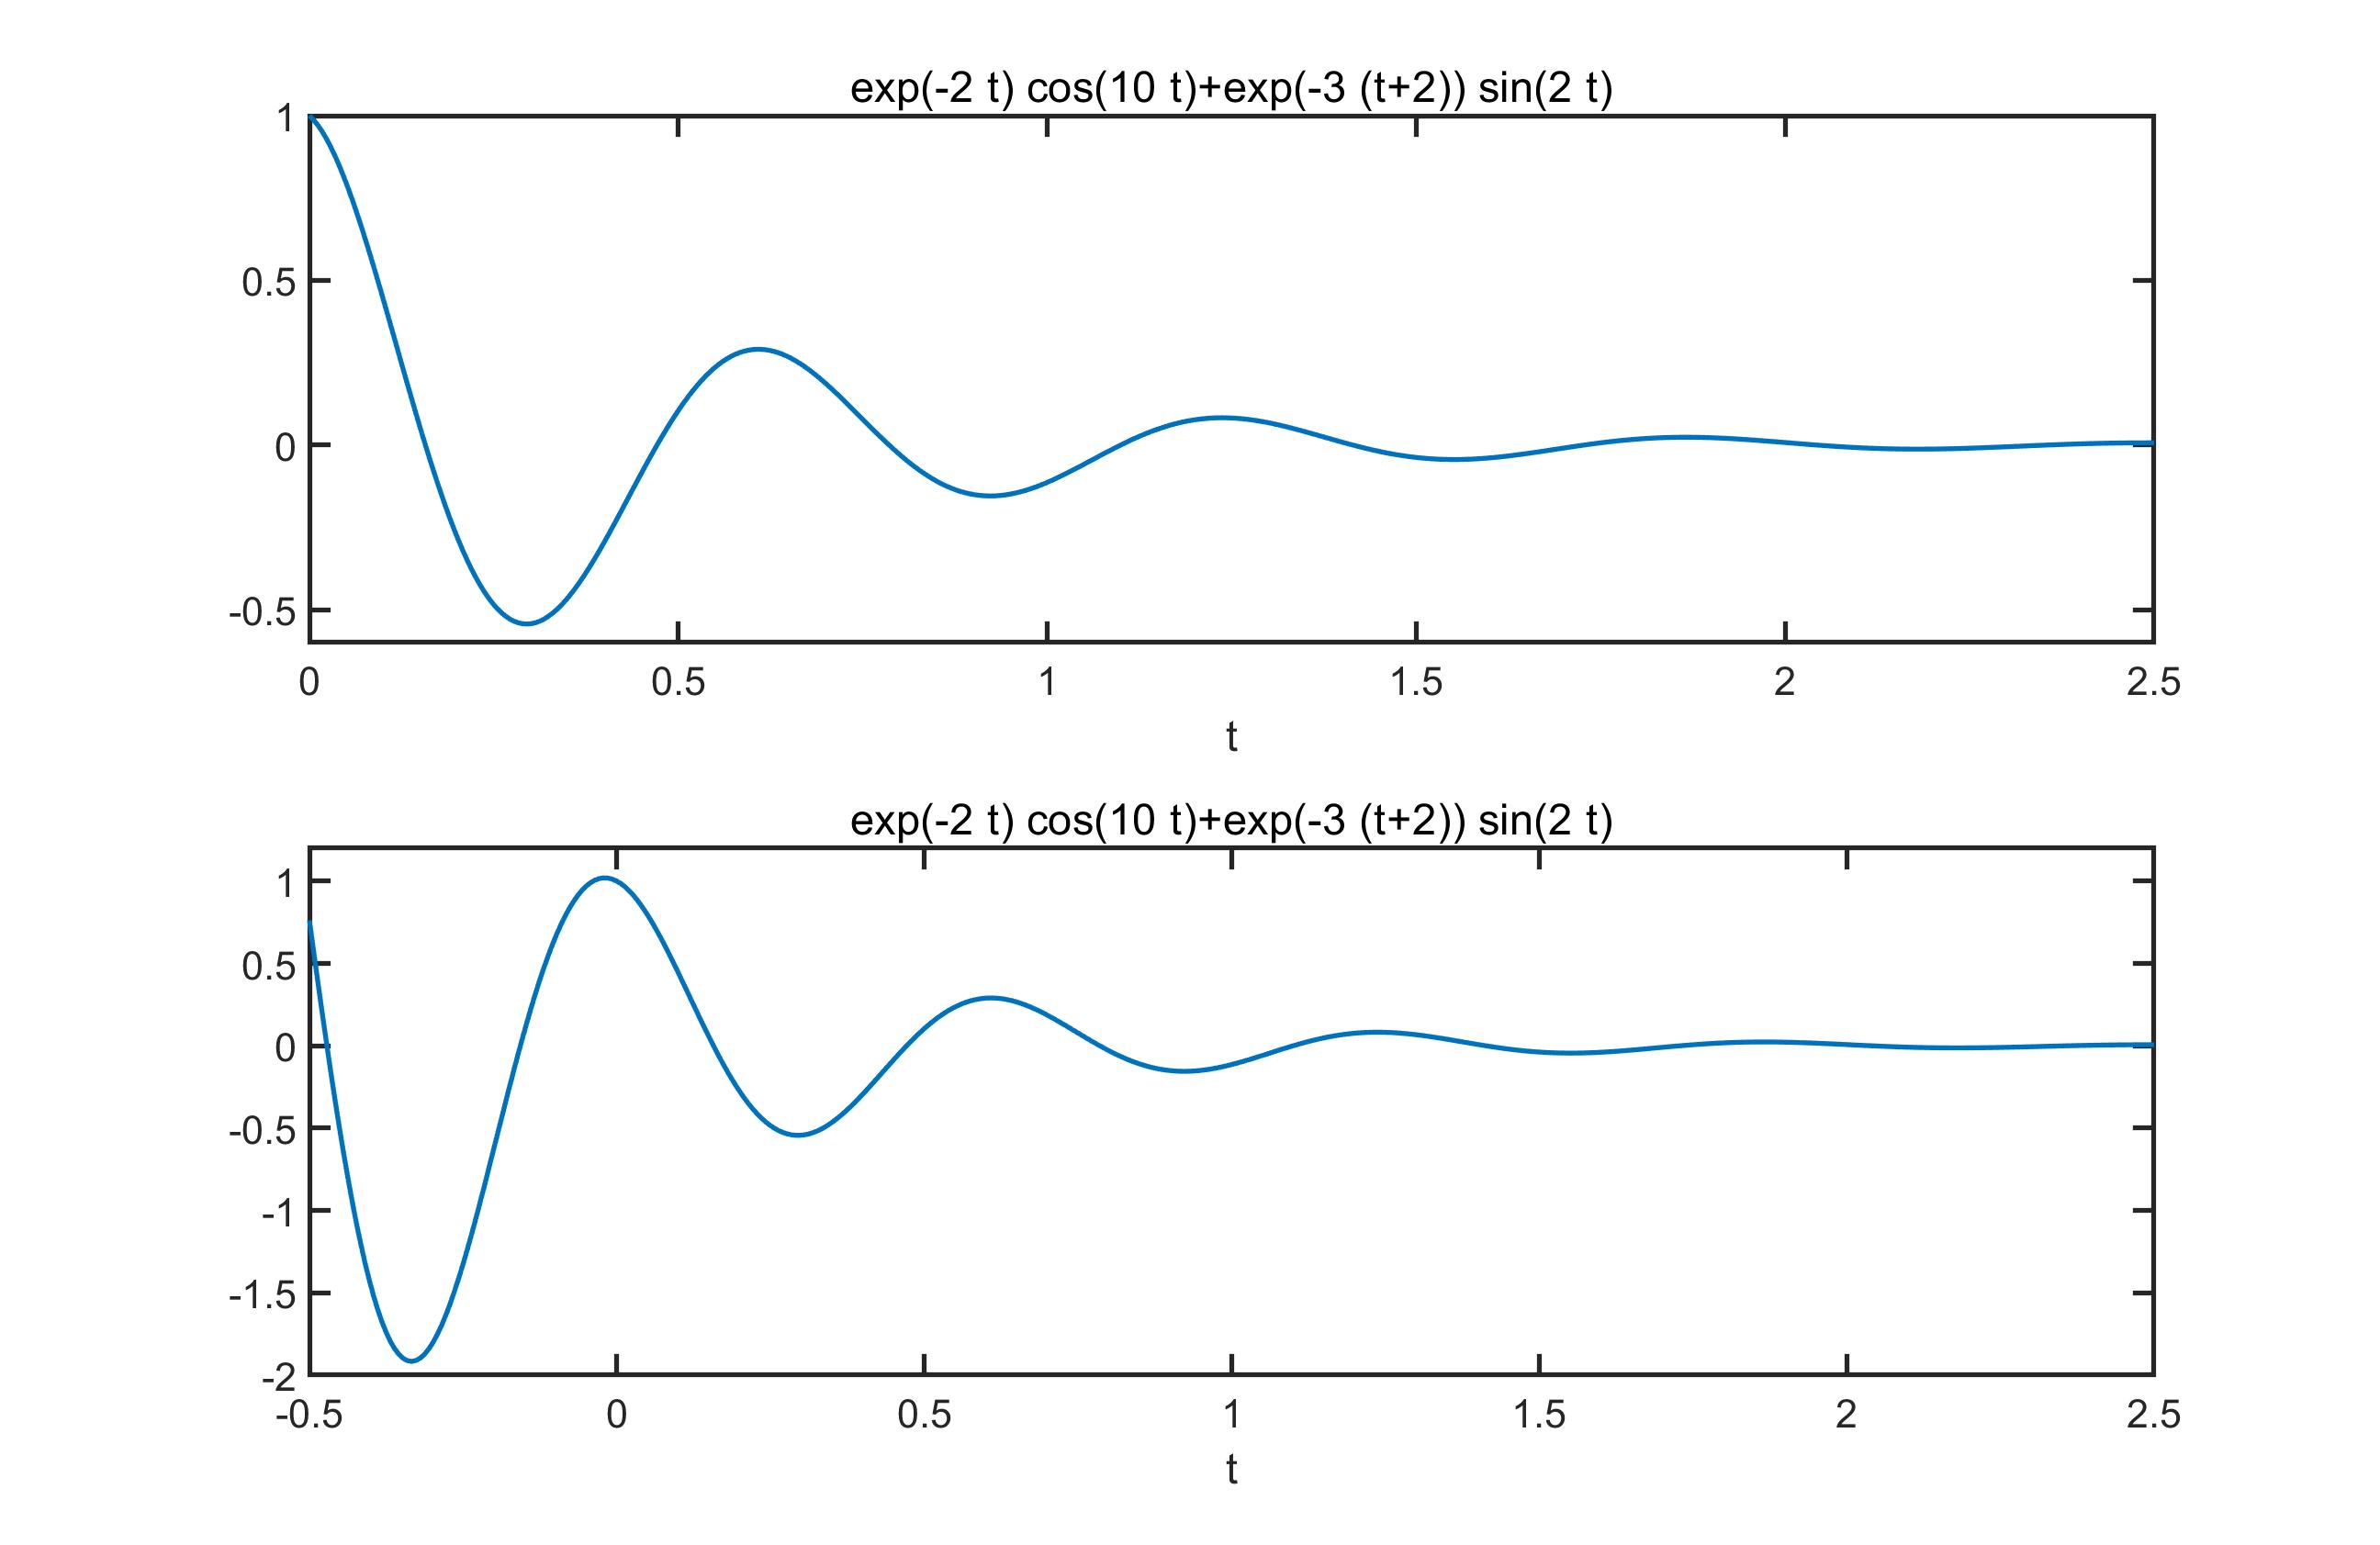
\includegraphics[width=.8\textwidth]{23}
			
	[t3\_1, f3\_1] =[0.9228, -0.1547] 初值t=1
	
	[t3\_2, f3\_2] =[0.2945, -0.5436] 初值t=.1
		\end{block}
		
	\end{columns}
\end{frame}
%---------------------------------------------------------------------- 
	\subsection{利用梯度求解最优化问题}
\begin{frame}[fragile]{利用梯度求解最优化问题}
\textbf{思路:}引入目标函数梯度,加快计算速度,改进搜索精度,但影响计算速度。即设置 optimset.GradObj='on' 。
	
	\begin{example}[6-14]
求解Rosenbrock函数$f\left(x_{1}, x_{2}\right)=100\left(x_{2}-x_{1}^{2}\right)^{2}+\left(1-x_{1}\right)^{2}$无约束最优化问题。
	\end{example}
	
	\begin{block}{MATLAB代码:}
\begin{lstlisting}
ff4=@(x)100*(x(2)-x(1)^2)^2+(1-x(1))^2;
ff4_0 = optimset; ff4_0.Display='iter'; ff4_0.TolX = 1e-10; ff4_0.TolFun= 1e-20;
x4 = fminunc(ff4,[0; 0],ff4_0)
syms x1 x2
ff4_1=100*(x2-x1^2)^2+(1-x1)^2;
J = jacobian(ff4_1,[x1, x2]);
\end{lstlisting}
	\end{block}				
\end{frame}
%---------------------------------------------------------------------- 
\begin{frame}[fragile]{利用梯度求解最优化问题}
	\begin{columns}[T]
		\column{.65\textwidth}
	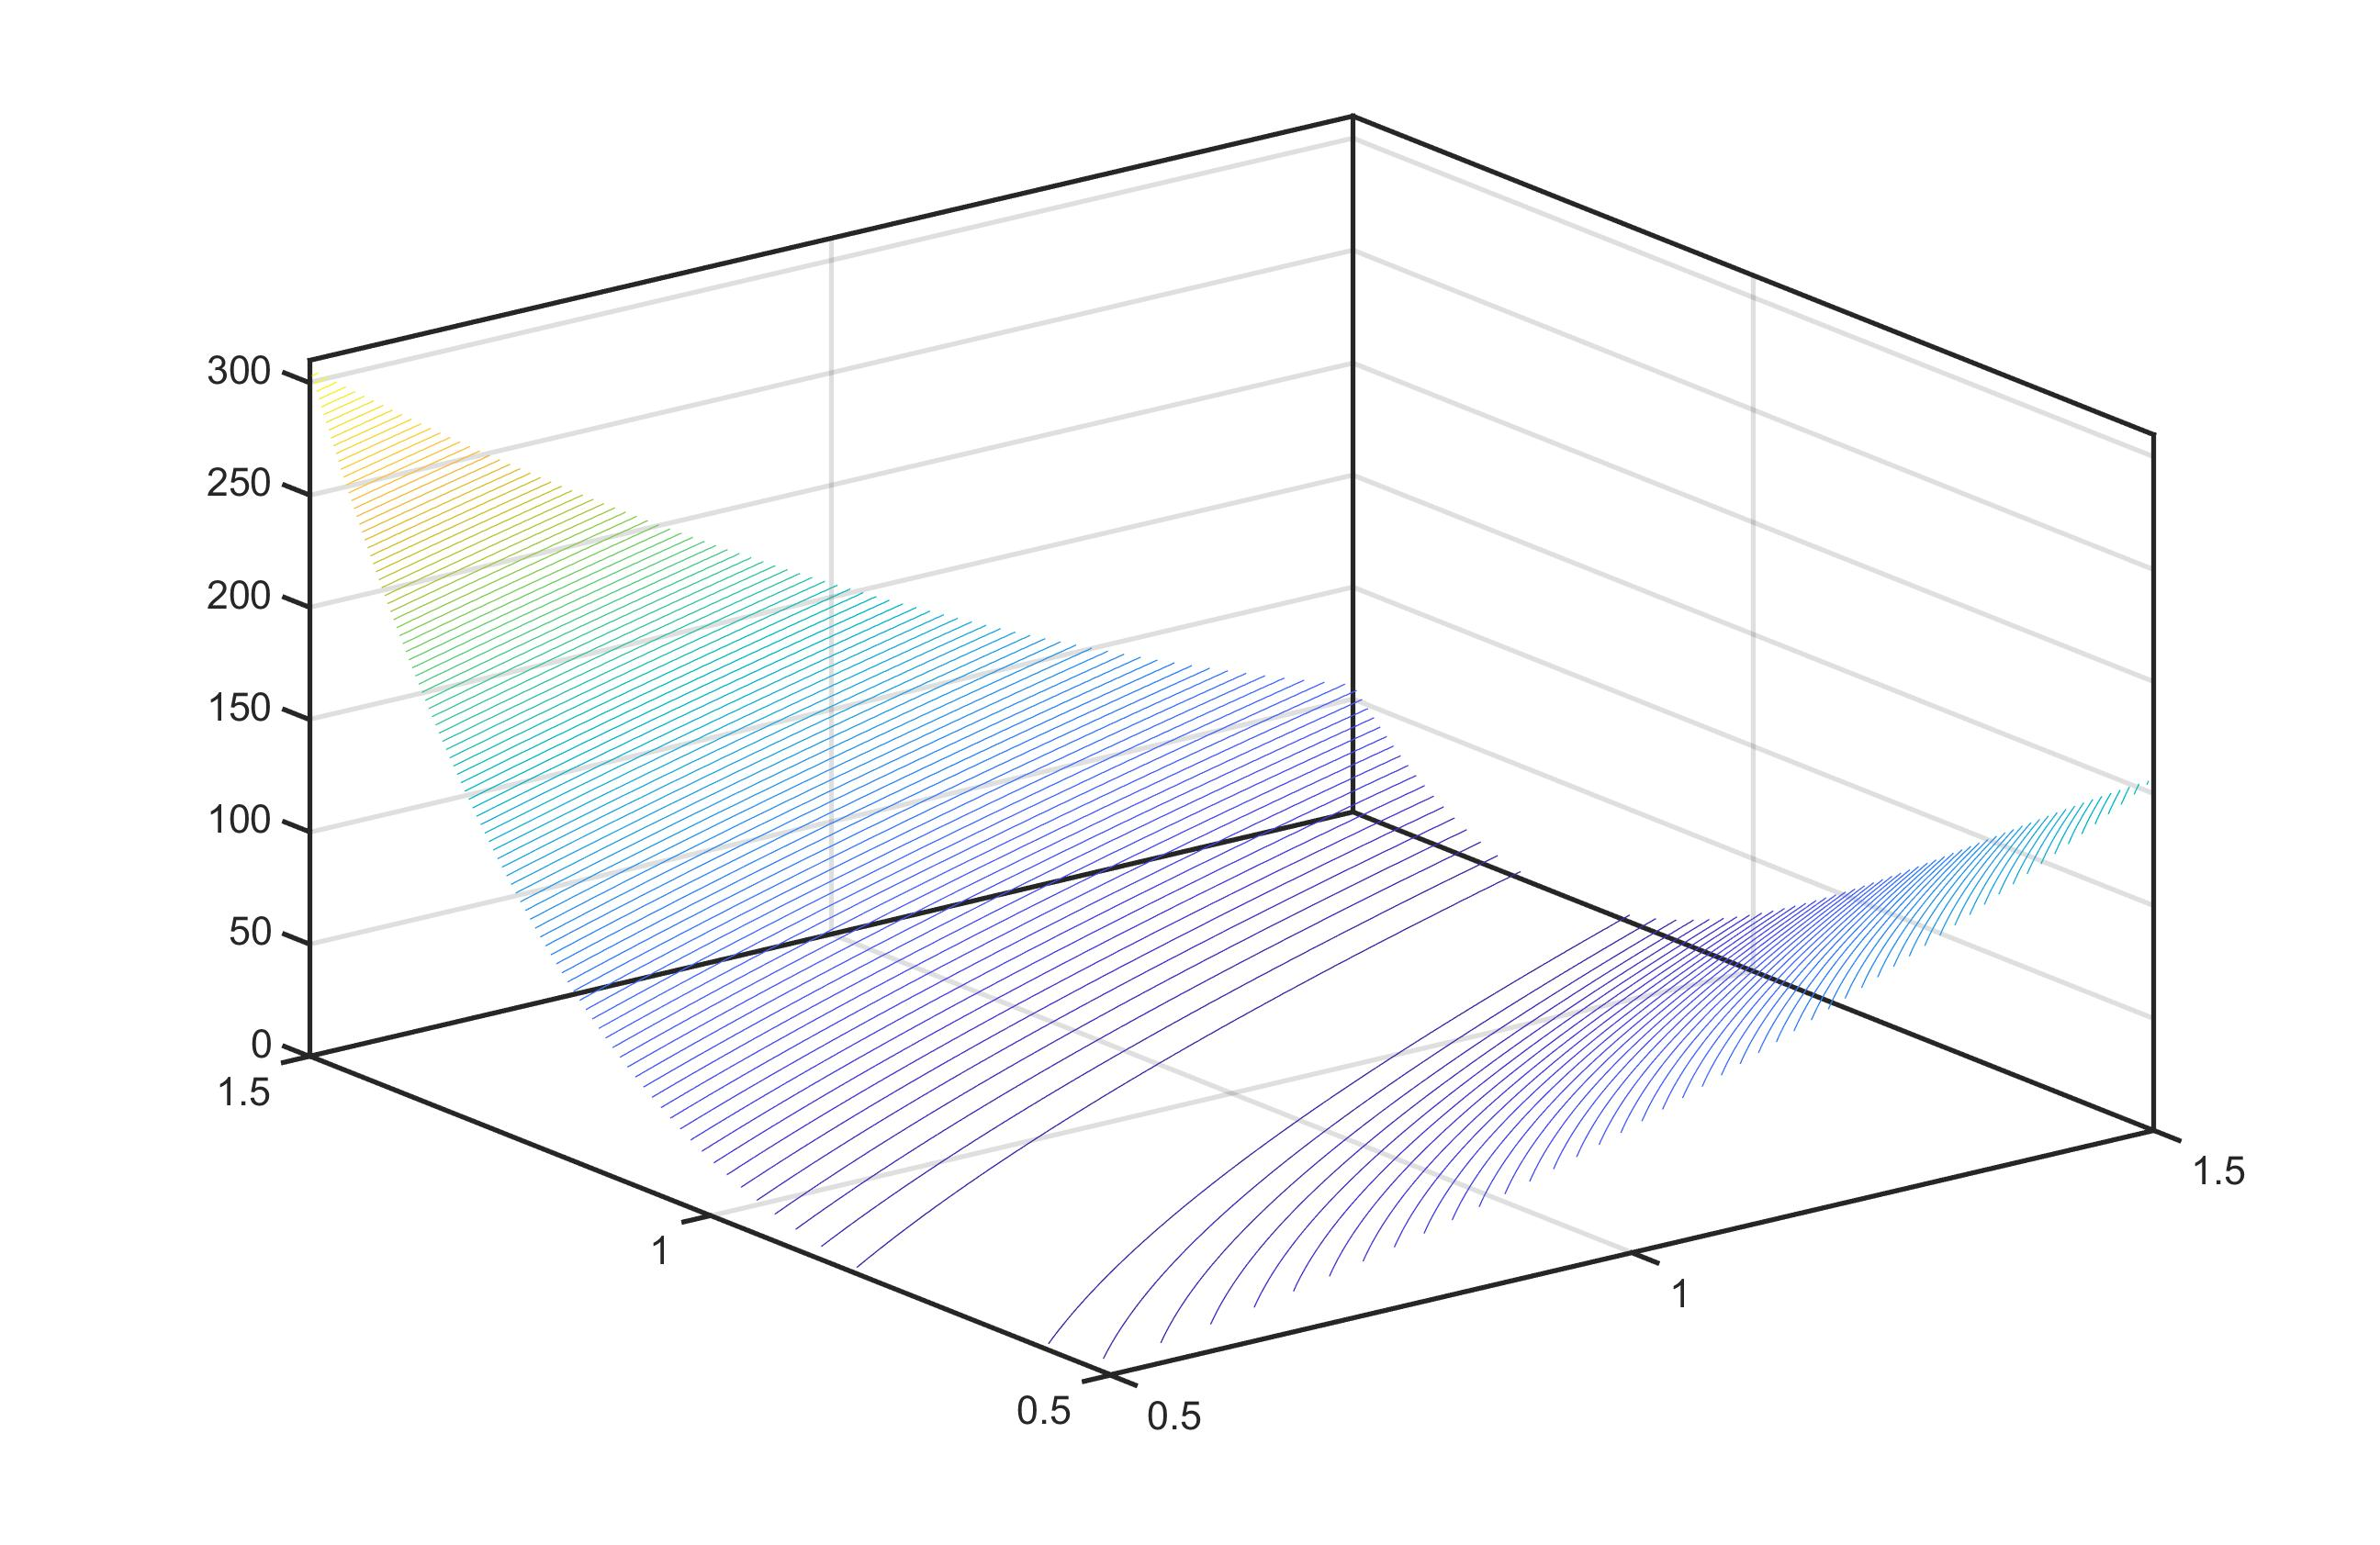
\includegraphics[width=\textwidth]{24}
		Rosenbrock函数,易知最小值(1,1)。

		\column{.4\textwidth}
\begin{block}{MATLAB代码(续):}
\begin{lstlisting}
ff4_0.GradObj='on';
x4_modi = fminunc(@ff4_modi,[0; 0],ff4_0)
function [y,Gy] = ff4_modi(x)
y = 100*(x(2)-x(1)^2)^2+(1-x(1))^2;
Gy = [2*x(1) - 400*x(1)*(- x(1)^2 + x(2)) - 2; - 200*x(1)^2 + 200*x(2)];
end
\end{lstlisting}
\end{block}	
	\end{columns}

\end{frame}
%---------------------------------------------------------------------- 
\begin{frame}[fragile]{利用梯度求解最优化问题}

\begin{lstlisting}                                            
Iteration  Func-count       f(x)        Step-size      First-order optimality
0           3                1                             2
1          12         0.771192      0.0817341           5.34  
......
20          81      1.94742e-11              1       1.06e-06
x4 = (1.0000,1.0000)
                   
Iteration  Func-count       f(x)        Step-size      First-order optimality
0           1                1                             2
1           4         0.771191      0.0817342           5.34  
......
22          29      1.16799e-23              1       1.26e-10
23          30      2.04561e-28              1       2.41e-13
x4_modi = (1.0000,1.0000)
\end{lstlisting}

\textbf{注:}实际情况常见带变量边界约束的最优化问题,如$\min\limits_{\mathbf{x}\ s.t.\ \mathbf{x_m} \leqslant \mathbf{x} \leqslant \mathbf{x_M}}$,可以调用fminsearchbnd()函数。

\end{frame}

%---------------------------------------------------------------------- 
\section{有约束最优化问题的计算机求解}
	\subsection{约束条件与可行解区域}
		\begin{frame}[fragile]{约束条件与可行解区域}
			\textbf{有约束最优化问题提法:}$\min\limits_{\mathbf{x}\ s.t.\ \mathrm{G}(\mathbf{x}) \leqslant \mathbf{0}} f(\mathbf{x})$。满足$\mathrm{G}(\mathbf{x}) \leqslant \mathbf{0}$的范围称为可行解区域(feasible region)。
			
		\begin{columns}[T]
	\column{.5\textwidth}
				
		\begin{example}[6-15]
			二元最优化问题$
			\begin{array}{l}
			\max \quad \left(-x_{1}^{2}-x_{2}\right)\\
			\left\{\begin{array}{l}
			9 \geqslant x_{1}^{2}+x_{2}^{2} \\
			x_{1}+x_{2} \leqslant 1
			\end{array}\right.
			\end{array}
			$
		\end{example}
				
	\begin{block}{MATLAB代码:}
\begin{lstlisting}
syms x1 x2
[x1,x2]=meshgrid(-3:.1:3);
z = -x1.^2 - x2;
i = find(x1.^2 + x2.^2 > 9);  z(i) = NaN;
i = find(x1 + x2 > 1);  z(i) = NaN;
surf(x1,x2,z)
\end{lstlisting}
	\end{block}	
				
	\column{.55\textwidth}
				
	\begin{block}{输出:}
\centering
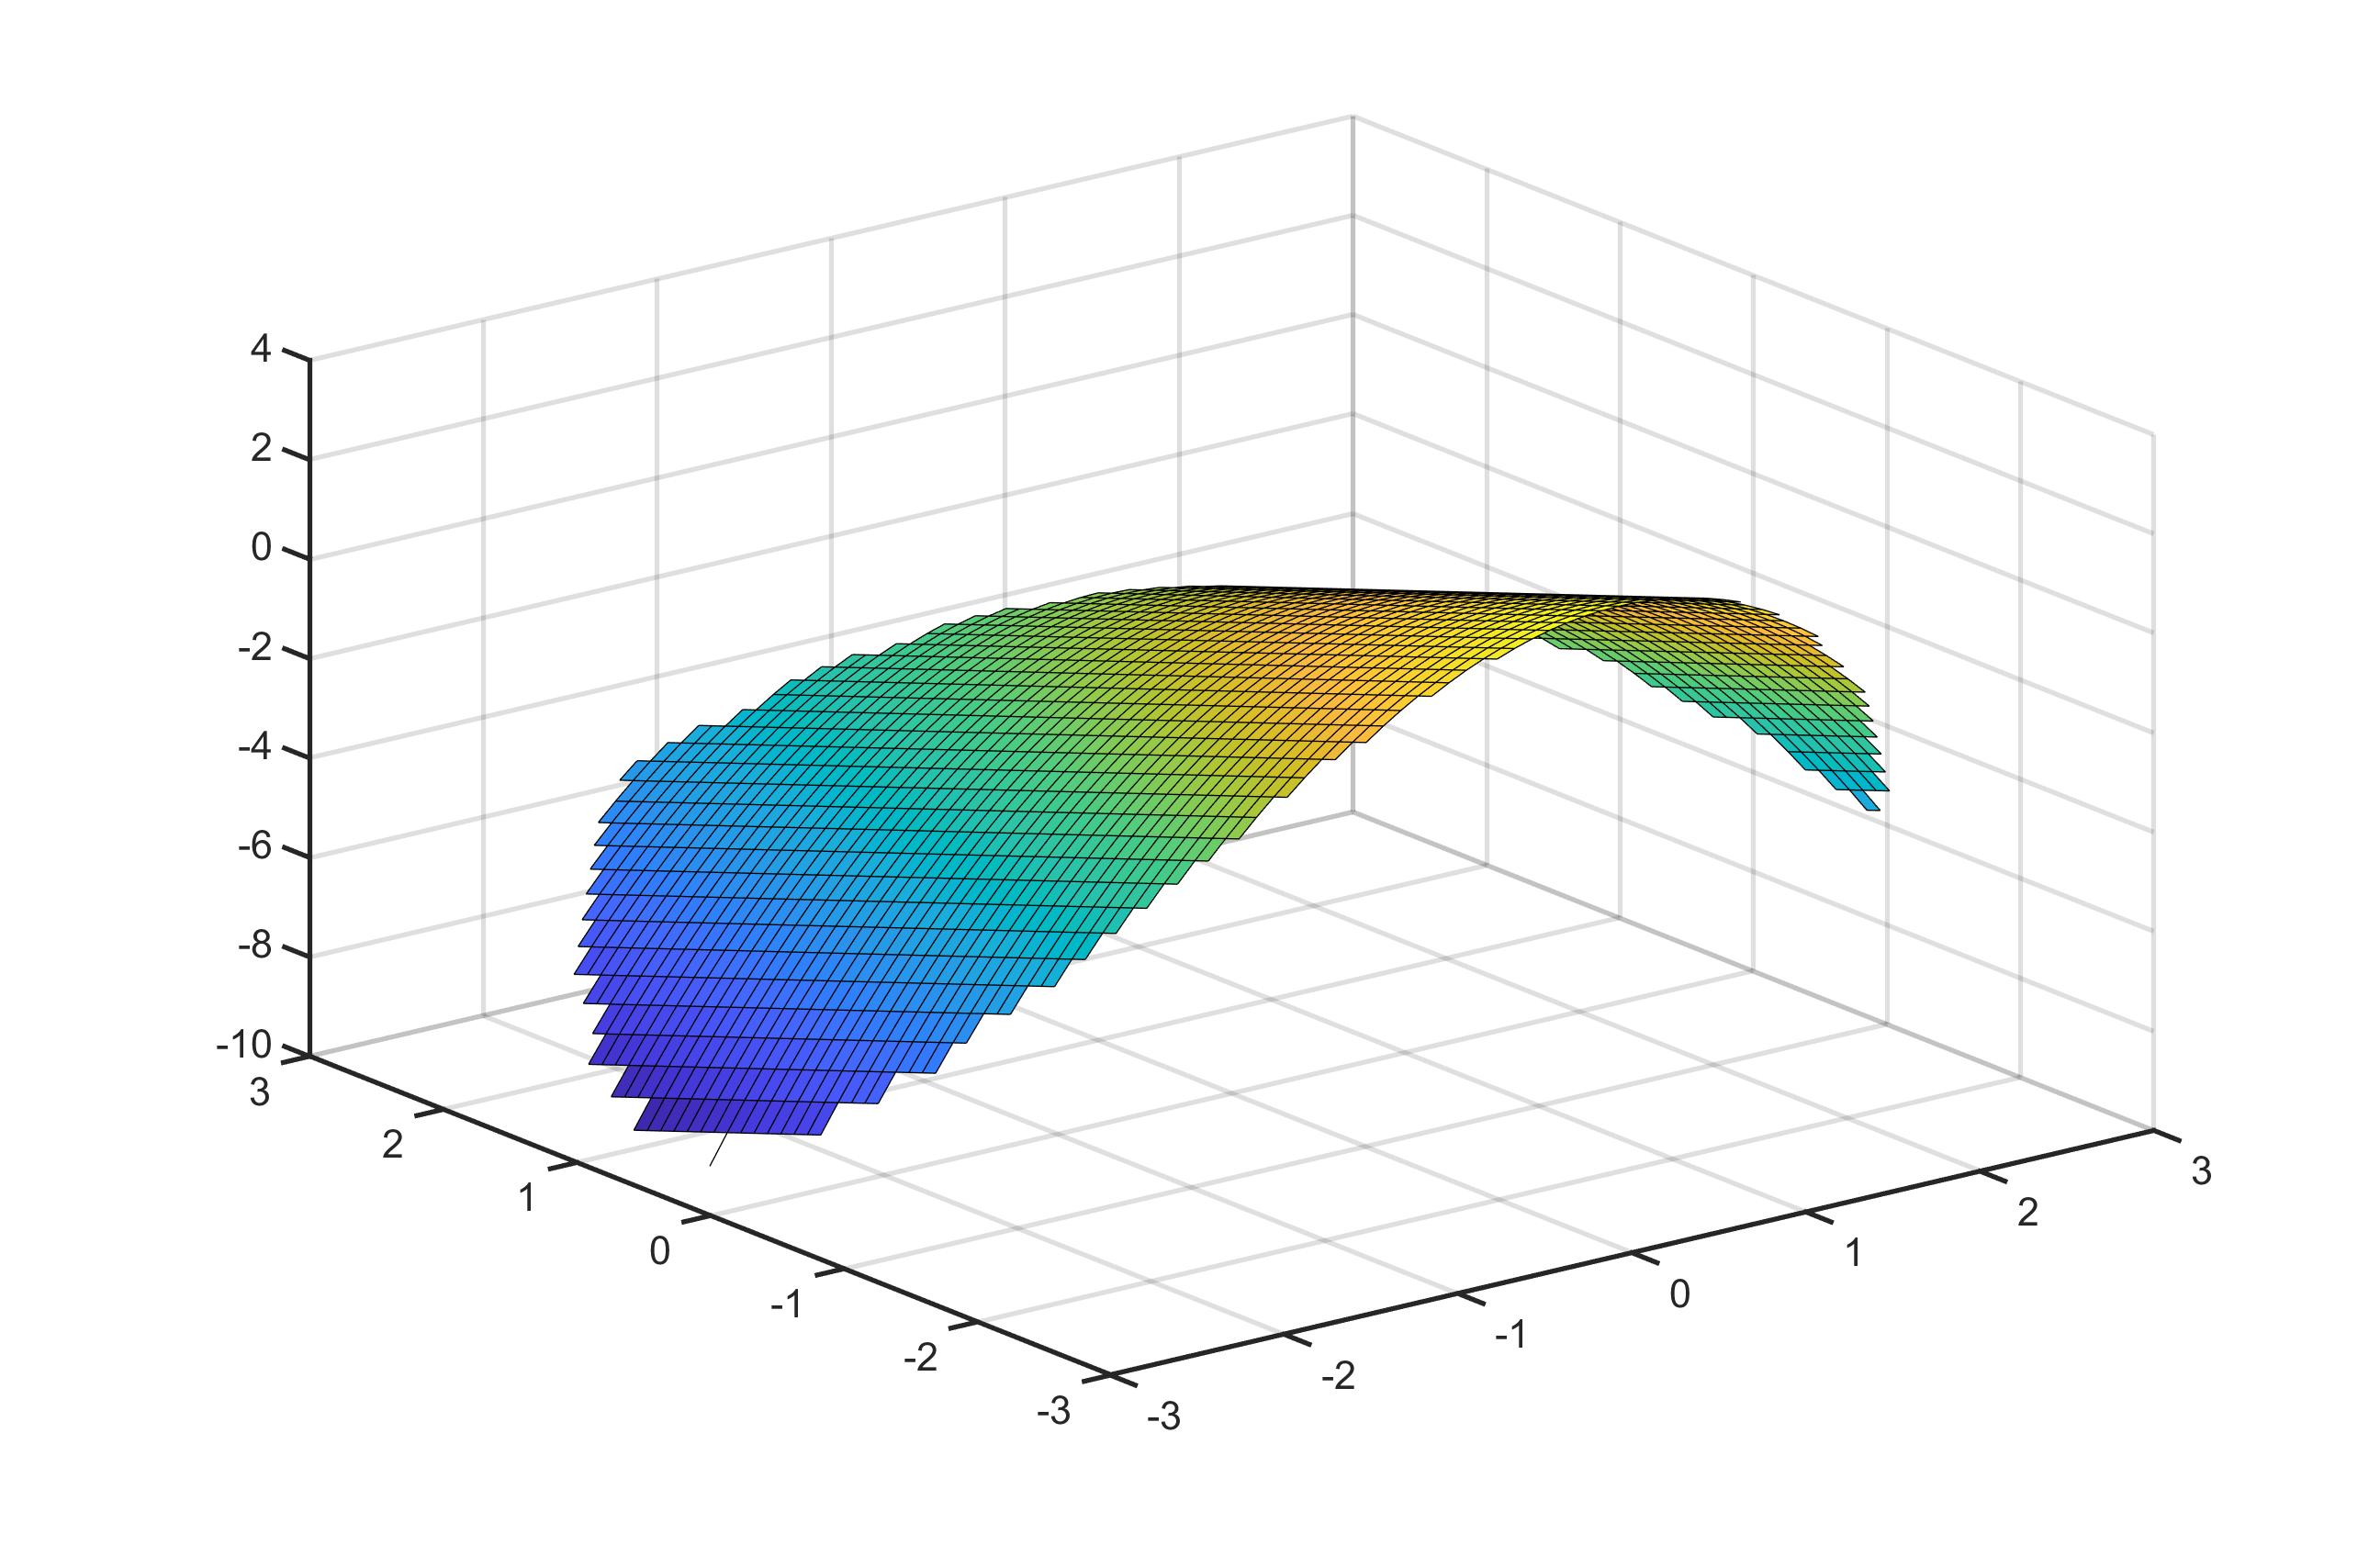
\includegraphics[width=\textwidth]{31}

max(z(:)) = 3,在(-3,0)处。
	\end{block}
		\end{columns}			
\end{frame}
%---------------------------------------------------------------------- 
	\subsection{线性规划问题的计算机求解}
\begin{frame}[fragile]{线性规划问题的计算机求解}
	\textbf{线性规划问题提法:}$
	\begin{array}{l}
	\min \quad \mathbf{f}^T \mathbf{x}\\
	\mathbf{x} \text { s.t. }\left\{\begin{array}{l}
	\mathbf{A} \mathbf{x} \leqslant \mathbf{B} \\
	\mathbf{A}_{\mathrm{eq}} \mathbf{x}=\mathbf{B}_{\mathrm{eq}} \\
	\mathbf{x}_{m} \leqslant \mathbf{x} \leqslant \mathbf{x}_{M}
	\end{array}\right.
	\end{array}$,
	
	线性不等式约束:$\mathbf{A} \mathbf{x} \leqslant \mathbf{B}$,线性等式约束:$\mathbf{A}_{\mathrm{eq}} \mathbf{x}=\mathbf{B}_{\mathrm{eq}}$,上界变量$\mathbf{x}_{M}$,下界变量$\mathbf{x}_{m}$。
	
	\begin{block}{linprog()函数调用:}
\begin{lstlisting}
[x,f_opt,flag,c] = linprog(f, A, B, A_eq, B_eq, x_m, x_M, x_0, OPT, p1, p2,...)
\end{lstlisting}
	\end{block}	
	
\end{frame}
%---------------------------------------------------------------------- 

\begin{frame}[t,fragile]{线性规划问题的计算机求解}

\begin{example}[6-17]
	$\begin{array}{l}
	\min \quad \left(-2 x_{1}-x_{2}-4 x_{3}-3 x_{4}-x_{5}\right)\\
	\mathbf{x} \text { s.t. }\left\{\begin{array}{l}
	2 x_{2}+x_{3}+4 x_{4}+2 x_{5} \leqslant 54 \\
	3 x_{1}+4 x_{2}+5 x_{3}-x_{4}-x_{5} \leqslant 62 \\
	x_{1}, x_{2} \geqslant 0,, x_{3} \geqslant 3.32, x_{4} \geqslant 0.678, x_{5} \geqslant 2.57
	\end{array}\right.
	\end{array}
	$
\end{example}

	\begin{columns}[T]
		\column{.5\textwidth}
			
	\begin{block}{MATLAB代码:}
\begin{lstlisting}
f = [-2;-1;-4;-3;-1]; A = [0 2 1 4 2; 3 4 5 -1 -1]; B = [54; 62];
Ae=[]; Be=[]; xm=[0 0 3.32 .678 2.57]; 
ff5_0 = optimset; ff5_0.LargeScale = 'off'; ff5_0.Display = 'iter';
ff5_0.TolX = 1e-15; ff5_0.TolFun = 1e-10; ff5_0.TolCon = 1e-9; 
[x, f_opt, key, c] = linprog(f, A, B, Ae, Be, xm, [], [], ff5_0)
\end{lstlisting}
	\end{block}	
			
		\column{.55\textwidth}
			
	\begin{block}{输出:}
\begin{lstlisting}
Iter = 2, Time = 0.013 ......

x =
19.7850
0
3.3200
11.3850
2.5700

f_opt = -89.5750
\end{lstlisting}
	\end{block}

	\end{columns}		

\end{frame}
%---------------------------------------------------------------------- 
	\subsection{二次型规划的求解}
		\begin{frame}[fragile]{二次型规划的求解}
	\textbf{二次型规划问题提法:}$
\begin{array}{l}
\min \quad \left(\frac{1}{2} \mathbf{x}^{\mathrm{T}} \mathbf{H} \mathbf{x}+\mathbf{f}^{\mathrm{T}} \mathbf{x}\right)\\
\mathbf{x} \text { s.t. }\left\{\begin{array}{l}
\mathbf{A} \mathbf{x} \leqslant \mathbf{B} \\
\mathbf{A}_{\mathrm{eq}} \mathbf{x}=\mathbf{B}_{\mathrm{eq}} \\
\mathbf{x}_{m} \leqslant \mathbf{x} \leqslant \mathbf{x}_{M}
\end{array}\right.
\end{array}$

	\begin{block}{quadprog()函数调用:}
\begin{lstlisting}
[x,f_opt,flag,c]=quadprog(H,f,A,B,A_eq,B_eq,x_m,x_M,x_0,OPT,p1,p2,...)
\end{lstlisting}
	\end{block}	

\begin{example}[6-18]
	$\begin{array}{l}
	\min \quad \left[\left(x_{1}-1\right)^{2}+\left(x_{2},+2\right)^{2}+\left(x_{3}-3\right)^{2}+\left(x_{4}-4\right)^{2}\right]\\
	\mathbf{x} \text { s.t. }\left\{\begin{array}{l}
	x_{1}+x_{2}+x_{3}+x_{4} \leqslant 5 \\
	3 x_{1}+3 x_{2}+2 x_{3}+x_{4} \leq 10 \\
	x_{1}, x_{2}, x_{3}, x_{4} \geqslant 0
	\end{array}\right.
	\end{array}
	$
\end{example}

\begin{block}{输出:}
	\begin{lstlisting}
Iter = 5...... x =(0.0000,0.6667,1.6667,2.6667); f_opt =-23.6667
	\end{lstlisting}
\end{block}	
			
		\end{frame}
%---------------------------------------------------------------------- 
	\subsection{一般非线性规划问题的求解}
\begin{frame}[fragile]{一般非线性规划问题的求解}
\textbf{一般非线性规划问题提法}$
\begin{array}{l}
	\min \quad f(\mathbf{x})\\
	\mathbf{x} \text { s.t. }\left\{\begin{array}{ll}
		\mathbf{A} \mathbf{x} \leqslant \mathbf{B} &, \mathbf{A}_{\mathrm{eq}} \mathbf{x}=\mathbf{B}_{\mathrm{eq}} \\
		\mathbf{x}_{m} \leqslant \mathbf{x} \leqslant \mathbf{x}_{M} &,\mathbf{C}(\mathbf{x}) \leqslant 0 \\
		\mathbf{C}_{eq}(\mathbf{x})= 0 &.
	\end{array}\right.
\end{array}$
	\begin{block}{fmincon()函数调用:}
\begin{lstlisting}
[x,f_opt,flag,c]=fmincon(F,x0,A,B,A_eq,B_eq,x_m,x_M,CF,OPT,p1,p2,...)
%全局最优解尝试,则调fmincon_global()函数,规则同上。
\end{lstlisting}
	\end{block}

\begin{example}[6-19]
$\begin{array}{l}
\min \quad \left[1000-x_{1}^{2}-2 x_{2}^{2}-x_{3}^{2}-x_{1} x_{2}-x_{1} x_{3}\right]\\
\mathbf{x} \text { s.t. }\left\{\begin{array}{l}
x_{1}^{2}+x_{2}^{2}+x_{3}^{2}-25=0 \\
8 x_{1}+14 x_{2}+7 x_{3}-56=0 \\
x_{1}, x_{2}, x_{3} \geqslant 0
\end{array}\right.
\end{array}
$
\end{example}
\end{frame}
%---------------------------------------------------------------------- 
\begin{frame}[fragile]{一般非线性规划问题的求解}
	\begin{block}{MATLAB代码}
\begin{lstlisting}
ff8_0 = optimset; ff8_0.LargeScale = 'off'; ff8_0.Display = 'iter';
ff8_0.TolX = 1e-15; ff8_0.TolFun = 1e-30; ff8_0.TolCon = 1e-20; 
x0=ones(3,1); xm=zeros(3,1); xM=[]; A=[]; B=[]; Aeq=[]; Beq=[];
[x,f_opt,flag,c] = fmincon(@opt_fun1, x0, A, B, Aeq, Beq, xm, xM, @opt_con1, ff8_0)
\end{lstlisting}		
	\end{block}	
	
	\begin{block}{输出}
\begin{lstlisting}
x =
3.5121
0.2170
3.5522

f_opt =
961.7152

iterations: 16
\end{lstlisting}		
	\end{block}	

\end{frame}
%----------------------------------------------------------------------	
\section{其他}
%	\subsection{应用实例}
%		\begin{frame}[allowframebreaks]{应用实例}
%		
%		\end{frame}
%---------------------------------------------------------------------- 	
	\subsection{学习心得}
		\begin{frame}[allowframebreaks]{学习心得}
	\textbf{一}\quad 这是本系统具体的书,可以了解,明白MATLAB能解决的问题,有实际需要时再详细翻阅。
	
	\textbf{二}\quad MATLAB集成很多科学计算算法,也方便调用。我联想到了FFTW、LAPACK等,让用户避免重复造轮子。
	但我认为需要对算法有些了解,定性明白它的长处和不足。
		\end{frame}

\end{document}